\chapter{\label{ch:introduction}Theory and Concepts}

\minitoc

\co{what this chapter is about}
%
In this chapter, I will explain the rationale and context for this thesis: can we fabricate graphene and, more broadly, graphene-derived structures that offer a competitive advantage over ubiquitous silicon integrated circuits? In an attempt to answer this question, I will present an overview of the key all-carbon alternatives studied so far since the late 1990s. This chapter begins with a concise overview of the microprocessor trend over the last few decades, followed by a discussion on fundamental properties of graphene, \glspl{CNT}, and \glspl{GNR}. Throughout the discussion, a selection of the most significant carbon-based proposals developed to date will be reviewed and critically analysed.

\section{The Path towards Carbon Electronics}\label{intro:sec:motivation}

\co{There is less Silicon around and it is incrementally difficult to maintain costs associated with its production}
Silicon has been the undisputed leader in the fabrication of \glspl{IC} for almost sixty years. The widespread shortage of semiconductors that began in late 2020, however, has prompted both major chipmakers and the scientific community to think more deeply and actively about which non-silicon technologies and materials are valid candidates for replacing or, more realistically, complementing silicon. Except for market leaders such as Intel, Samsung and TSMC, long-term manufacturing costs remain largely expensive.

In 2021, Bloomberg reported that the fundamental costs of constructing a semiconductor manufacturing are approximately \$15 billion, with profit requirements of roughly \$3 billion to maintain market competition and avoid obsolescence~\cite{king2021}. These findings are also backed by a study last year conducted by the Boston Consulting Group, which ranked investments in research and development (22\% of annual semiconductor sales) and capital spending (26\%) as the highest in all industries~\cite{veras2021}.

\co{The success of CMOS is in the density scaling}
The first prototype of a point-contact transistor, developed at the beginning of the 1940s by Bardeen, Brattain and William Shockley at Bell Labs, and the creation of \gls{CMOS} techology by Atalla and Kahng ten years later, together marked the beginning of integrated components~\cite{shockley1984path}.
Arguably, the density-scaling capabilities of this technology has been one of the main reasons responsible for the constant technological development over a time span of more than fifty years. In this scenario, Moore's law is considered both as a metric for estimating future numbers of transistors per integrated circuit and also as a driver of innovation and competitiveness.

\co{One of the problem of the advancement of modern IC is the scaling limitations of CMOS}
The search for new materials for integrated electronics is not only related to increase the number of transistors per chip. Fig.~\ref{fig:intro:moore_law} displays five microprocessor figures of merit and their trends over the past five decades. The clock frequency is the number of clock cycles (number of electrical pulses) that a CPU can execute every second and is measured in \si{\Hz}. Within these electrical pulses, the CPU can conduct fundamental operations such as memory access, data writing, and instruction retrieval, and generates heat. From Fig.~\ref{fig:intro:moore_law} it is clear that a positive correlation exists between the clock speed and the power dissipated\footnote[2]{This is typically referred as static power, i.e.\ power dissipated when the transistor is not switching. \Gls{CMOS} technology is well known for low static power for standard supply voltages (\SIrange{3}{5}{\volt})}, and this has been one of the main reasons that has motivated, for example, the research of materials with high thermoelectric-conversion efficiency~\cite{gemma2021roadmap, dresselhaus2007new}.

\begin{figure}[hbtp]
    \begin{center}
        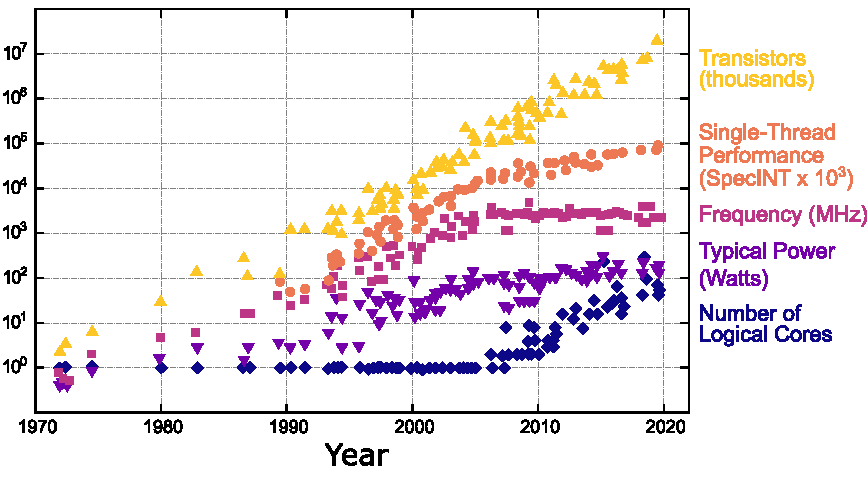
\includegraphics[width=\textwidth]{chapter_introduction/figures/moore.pdf}
        \caption[Moore's Law for Microprocessors]
        {
            The arc of Moore's law over fifty years of microprocessor development. While the number of transistors have doubled about every two years, the same cannot be said for other key figures. In particular, clock frequency and power dissipated have plateaued out since 2003. The release in 2005 by Intel of the first dual-core processor (Pentium D), and the ability to perform hyper-threading have sparked reserach into the number of logical cores per CPU. This is the ability of a single core to carry out two or more processes simultaneously. Since then, the increase in multi-threading performance compared with stagnating single-thread performance has been one of the main driving factors for multi-core processors in modern laptops. Data collected by K.\ Rupp. Adapted from a talk given by Nvidia.
        }
        \label{fig:intro:moore_law}
    \end{center}
\end{figure}
%
One of the major problematics with the \gls{CMOS} density scaling is that as the channel length is shortened, leakge current increases because of quantum tunneling of the charge carriers through the channel. This issues has been mitigated over the last few years by adopting non-planar transistor architectures such as FinFETs~\cite{yang20045nm} and Gate-All-Around FETs~\cite{gu2011first}, but fundamental problems still remains.

Several researchers have envisioned graphene as one of the most robust materials against short-channel effects~\cite{neumaier2019integrating, chaudhry2004controlling, xie2012review, feijoo2016short,schwierz2010graphene, thiele2010modeling} and suggested that it will be possible to integrate graphene into semiconductor manufacturing cycles in the near future. In order to understand the rationale of such proposals, in the next section we will outline some of the fundamentals properties of graphene and how they have been used in \gls{CMOS} prototypes.

\section{Graphene}\label{intro:sec:graphene}

\subsection{Crystal and Band Structure}
Graphene has a hexagonal structure, where the carbon atoms are hybridised as $sp^2$. In the International Table of Crystallography, graphene is included in the symmorphic space group \#191, with symmetry $D_{6h}$ ($P6/mmm$)~\cite{dresselhaus2007group}.

As shown in Fig.~\ref{fig:intro:graphene_lattice}a--b, the carbon atoms in graphene form a two-dimensional hexagonal lattice with two non-equivalent atoms per unit cell:
%
\begin{equation}\label{eq:graphene_lattice_vectors}
    \vect{a}{_1} = \frac{a}{2}(3, \sqrt{3}),~
    \vect{a}{_2} = \frac{a}{2}(3, -\sqrt{3}),
\end{equation}
%
with $a\simeq\SI{1.42}{\angstrom}$ the carbon--carbon bond length.
Each atom belonging to one sublattice, called sublattice A, has three nearest neighbours belonging to the other sublattice, called sublattice B. With respect to one atom chosen from sublattice A as origin, the position of these first three neighbours in real space are given by:
%
\begin{equation}\label{eq:graphene_first_neighbours}
    \vect{\updelta}{_1} = \frac{a}{2}(1, \sqrt{3}),~
    \vect{\updelta}{_2} = \frac{a}{2}(1, -\sqrt{3}),~
    \vect{\updelta}{_3} = -a(1,0),
\end{equation}
%
while the reciprocal-lattice vectors may be written as:
%
\begin{equation}\label{eq:graphene_reciprocal_vectors}
    \vect{b}{_1} = \frac{2\pi}{3a}(1, \sqrt{3}),~
    \vect{b}{_2} = \frac{2\pi}{3a}(1, -\sqrt{3}).
\end{equation}
%
% In order to define the vertices of the Brillouin zone, one has to apply the Bragg condition:
%
% \begin{equation}\label{eq:Bragg}
%     2\vect{k}\cdot\vect{G} = 0,
% \end{equation}
% %
% where
% %
% \begin{equation}
%     \vect{G} = n\vect{b}_1 + m\vect{b}_2.
% \end{equation}
% %
% The first amongst these vertices are:
% %
% \begin{align*}
%     n & = \pm 1, & m & =0,     & \vect{G} & =\pm\vect{b}_1,              \\
%     n & = 0,     & m & =\pm 1, & \vect{G} & =\pm\vect{b}_2,              \\
%     n & = \pm 1, & m & =\pm 1, & \vect{G} & =\pm(\vect{b}_1+\vect{b}_2),
% \end{align*}
% %
% and all these vectors have the same length $\abs{\vect{G}} = \frac{4\pi}{3a}$. By applying the Bragg condition in the first of the three cases we obtain
% %
% \begin{equation}
%     \sqrt{3}k_{x} + k_{y} = \mp~\frac{4\pi}{3a},
% \end{equation}
% %
whereas the Brillouin point are:
%
\begin{align}\label{eq:K_point_components}
    \vect{K}  & \equiv\mp~\frac{2\pi}{3a}\qty(\frac{1}{\sqrt{3}}, 1),  \\
    \vect{K'} & \equiv\pm~\frac{2\pi}{3a}\qty(\frac{1}{\sqrt{3}}, -1), \\
    \vect{M}  & \equiv\pm\qty(0, \pm~\frac{2\pi}{3a}).
\end{align}
%
Based on the experimental evidence collected in the last 20 years, the model that best describe the properties of graphene is the Wallace model of the band structure, which dates back to 1947, and qualifies graphene as a semimetal with a linear dispersion of the electronic excitations close to the Fermi energy~\cite{wallace1947band}.

\begin{figure}
    \begin{center}
        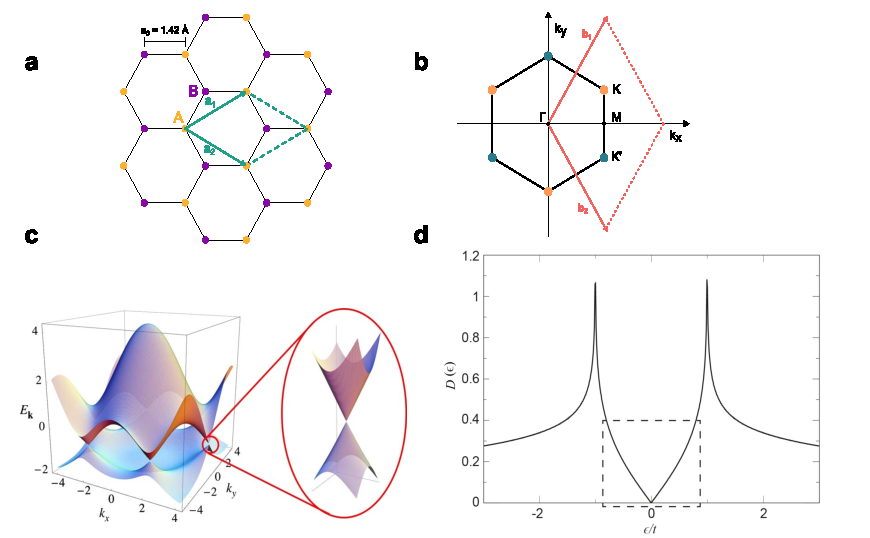
\includegraphics[width=0.95\columnwidth]{chapter_introduction/figures/graphene_lattice.pdf}
        \caption[Honeycomb Lattice, Dirac Cones, and Graphene Density of States]
        {
            \textbf{a}, Honeycomb lattice of graphene. Two non-equivalent carbon atoms A and B in the primitive cells (direct space) are denoted in yellow and purple. The set of possible translations are shown by the lattice vectors $\vect{a}_1,\vect{a}_2$ (green arrows).
            \textbf{b}, The first Brillouin zone of graphene with vertices \vect{K} (orange) and \vect{K$'$} (green), and reciprocal-lattice vectors drawn in red.
            \textbf{c}, Graphene energy dispersion resulting from Eq.~\ref{eq:graphene_hamiltonian} (in units of the hopping parameter $t$). The magnification shows one of the Dirac cones, which are located at the \vect{K} and \vect{K$'$} points, emphasising the linear-dispersion relation.
            \textbf{d}, The electron states density as a function of $t$, showing pronounced van Hove singularities for $\varepsilon\simeq \pm t$. The dashed rectangle indicates the low-energy linear-dispersion region which is typically probed in transport experiments.
            Adapted from~\cite{castroneto2009}.
        }
        \label{fig:intro:graphene_lattice}
    \end{center}
\end{figure}

Within the second-quantization formalism (with $\hbar = 1$), the tight-binding Hamiltonian may be written as
%
\begin{equation}\label{eq:graphene_hamiltonian}
    \mathcal{H}_\textrm{TB} = -t\sum_{\langle ij\rangle,\sigma}\qty(a^\dagger_{\sigma,i}b_{\sigma,j} + \textrm{h.c.}) - t' \sum_{\langle\langle ij\rangle\rangle,\sigma}\qty(a^\dagger_{\sigma,i}a_{\sigma,j}+b^\dagger_{\sigma,i}b_{\sigma,j}+ \textrm{h.c.}),
\end{equation}
%
The notation $\langle ij\rangle$ means the sum runs over pairs of electrons that are nearest neighbours; similarly, the notation $\langle\langle ij\rangle\rangle$ specifies a summation over the next-nearest neighbours. The two operators $a^\dagger_{i,\sigma}$ ($a_{i,\sigma}$) and $b^\dagger_{i,\sigma}$ ($b_{i,\sigma}$) create (annihilate) an electron with spin $\sigma=~\uparrow,\downarrow$ for atoms on sublattices A and B, respectively. The value of $t$ that best reproduces the experimental evidence is $t\simeq2.8$ \si{\electronvolt}~\cite{castroneto2009}, and quantifies the nearest-neighbour hopping energy; similarly, $t'$ denotes the next-nearest-neighbour hopping energy, and the experimental estimate is $t'\simeq\SI{0.1}{\electronvolt}$~\cite{deacon2007cyclotron}.

By diagonalising the Hamiltonian in Eq.~\ref{eq:graphene_hamiltonian}, it is possible to work out the energy dispersion of graphene,
%
\begin{equation}\label{intro:sec:graphene:eq:energy_bands}
    E_{\pm}(\vect{k}) = \epsilon_p - t'f(\vect{k}) \pm t\sqrt{3 + f(\vect{k})},
\end{equation}
%
with $f(\vect{k})$ defined as:
%
\begin{equation}\label{intro:sec:graphene:eq:energy_bands_fk}
    f(\vect{k})=2\cos{\left(\sqrt{3}k_ya\right)} + 4\cos{\qty(\frac{\sqrt{3}}{2}k_ya)}\cos{\qty(\frac{3}{2}k_xa)}.
\end{equation}
%
Eq.~\ref{intro:sec:graphene:eq:energy_bands} identifies an upper band ($\pi^*$) associated with the plus sign and a lower band ($\pi$) associated with the minus sign, and these bands are symmetric with respect to zero energy\footnote[3]{The fact that the energy dispersion is symmetric to zero energy is a result of the particle--hole symmetry of the system.}. If the system is undoped, there will be one electron per carbon atom, resulting in two electrons per cell: the lower band will be full, while the top band will be empty. Therefore, the system is semi-metallic.

When examining the trend close to the \vect{K} and \vect{K$'$} points, the peculiarities of the energy-band dispersion can be appreciated. By taking the positive components for the \vect{K} point, as defined in Eq.~\ref{eq:K_point_components}, and expanding Eq.~\ref{intro:sec:graphene:eq:energy_bands} as $\vect{k} = \vect{K} + \vect{q}$, with $\abs{(\vect{q})}\ll\abs{(\vect{K})}$, one obtains:
%
\begin{equation}
    E_{\pm}(\vect{q}) = \epsilon_p \pm \frac{3at}{2}\abs{\vect{q}},
\end{equation}
%
This remarkable result tells us that the dispersion close to the Fermi level is linear in \vect{q}. The Fermi velocity is defined by the usual relation $v_F = \frac{1}{\hbar}\qty(\dv{E}{\vect{k}})$, and in graphene $v_F\simeq1\times 10^6~\textrm{ms}^{-1}$~\cite{wallace1947band}. An important consequence of this result is that while for a two-dimensional electron gas the \gls{DOS} is constant, the \gls{DOS} in graphene close to the Fermi level is:
%
\begin{equation}\label{eq:grafene:density_of_states}
    \rho(E)=\frac{2A_\textrm{cell}}{\pi}\frac{\abs{E}}{v_F^2}.
\end{equation}
%
This linear dependency of the electronic states density on the absolute value of the energy has important consequences on the particle velocity $c^* = v_F = 3ta/2\hbar$, which is constant and similar to the speed of light $E = pc = c^*\hbar\abs{\vect{k} - \vect{K}}$~\cite{wolf2014graphene}. This similarity has led to the definition of \textit{massless fermions} for electrons near the Fermi energy of graphene~\cite{novoselov2004electric}. Furthermore, for undoped graphene, the \gls{DOS} displays two Van Hove singularities at $\rho(\omega_\textrm{VH}) = \pm\SI{1}{\electronvolt}$~\cite{bena2005quasiparticle}. This behaviour is rather different to the conventional case of electrons in 2D metals, where they have energy dispersion $\epsilon=\hbar^2 q^2 / 2 m^*$ in terms of the band mass $m^*$, and where one obtains a constant density of states $\rho^\textrm{2D}(\epsilon)=g m^* / 2 \pi \hbar^2$.

Finally, the graphene conductivity may be computed semiclassically using the Einstein--Smoluchowski relation\footnote[2]{$D = k_\textrm{B}T/\eta = \mu k_\textrm{B}T$, where $k_\textrm{B}T$ is the thermal energy of a flow of semiclassical charge carriers that experience an average friction coefficient $\eta$ when diffusing in a medium with coefficient $D$.} and the \gls{DOS}~\cite{bolotin2008temperature}:
%
\begin{equation}\label{ch1:eq:semiclassical_conductivity}
    \sigma_{\textrm{sc}}=e^{2} \rho v \ell_{\mathrm{el}},
\end{equation}
%
where $v$ is the carrier velocity, $\ell_{\mathrm{el}}$ the elastic mean free path (see Ch.~\ref{ch:theory}), and $e$ the elementary charge. From Eq.~\ref{ch1:eq:semiclassical_conductivity} and by knowing the charge density $n$, one can calculate the charge mobility, which at $T=\SI{0 }{\kelvin}$ reads:
%
\begin{equation}
    \mu(E)=\frac{\sigma_\mathrm{sc}}{e n}.
\end{equation}
%
Close to the Dirac points, the experimental conductivities lie within $\sigma\simeq 2-5~e^{2}/ h$~\cite{chen2008charged}, although several experiments have demonstrated a variation of more than an order of magnitude because of doping from the electrical contancts or the substrate~\cite{jiang2007quantum, ozyilmaz2007electronic}.


\subsection{Graphene Transistors}

The remarkable properties outlined in the last section are certainly amongst the reasons that motivates the great emphasis put on graphene in the 2021 International Roadmap for Devices and Systems~\cite{neisser2021international}, which in its \textit{beyond CMOS} study analyses technologies and semiconductor materials that will supplement or replace silicon (Tab.~\ref{intro:tab:graphene}).

\begin{table}
    \centering
    \begin{tabular}{l*{7}{c}}
        \toprule
                                                               & \multicolumn{3}{c}{Direct Gap} & \multicolumn{2}{c}{Indirect Gap}\T\B                                              \\
        \cmidrule(lr){2-4} \cmidrule(lr){5-6}
                                                               & InP                            & Si                                   & Ge   & GaAs  & InAs   & Graphene    \T\B   \\
        \midrule
        $a_\textrm{lattice}$ (\si{\angstrom})                  & 5.87                           & 5.43                                 & 5.65 & 5.65  & 6.06   & 2.46           \T  \\
        $E_g$ (eV)                                             & 1.35                           & 1.12                                 & 0.66 & 1.42  & 0.36   & 0               \T \\
        $\mu$ (cm$^2$V$^{-1}$s$^{-1}$) at 300 K                & 2800                           & 1400                                 & 3900 & 4600  & 16,000 & 200,000         \T \\
        $v_\textrm{sat}$ ($10^7$ \si{\centi\metre\per\second}) & 2.2                            & 1                                    & 0.6  & 2.2   & 4.0    & \textgreater{}5 \T \\
        DOS ($m^*/m_0$)                                        & 0.077                          & 1.08                                 & 0.56 & 0.067 & 0.023  & 0               \T \\
        $\epsilon_r$                                           & 12.4                           & 11.9                                 & 16.0 & 13.1  & 14.6   & 2.4             \T \\
        $\kappa$ (\si{\watt\per\metre\per\kelvin})             & 68                             & 150                                  & 60.2 & 46    & 27     & 5000            \T \\
        \bottomrule
    \end{tabular}
    \caption{Comparison between graphene and the most common materials in semiconductor electronics. The general interest in finding solutions for circumventing the absence of the bandgap in graphene is due to various graphene characteristics, including mobility, carrier velocity at saturation, low electrostatic shielding provided by a very low dielectric constant, and an excellent ability to conduct heat, as shown by thermal conductivity values. The last point is particularly pertinent to the design of graphene-based thermal sinks.}\label{intro:tab:graphene}
\end{table}

Initial interest for using graphene as a channel material in \gls{CMOS} logic may have been fueled by its remarkable mobility~\cite{schwierz2010nanometer}. In a standard CMOS gate, carriers are driven by a longitudinal electric field $\CMcal{E}_\textrm{SD}$ from the the source to the drain, and their motion is often limited by various scattering sources, such as collisions between electrons and phonons of the crystal lattice from which the gate is made. In their first graphene-based \gls{FET} prototype, Novoselov and colleagues measured an impressive intrinsic mobility $\mu_e^{\textrm{in}}$ at \SI{290}{\kelvin} close to $\mu_e^\textrm{in}\simeq10,000$ cm$^{2}$V$^{-1}$s$^{-1}$~\cite{novoselov2004electric} using a single layer of graphene on a \ce{Si}/\ce{SiO2} substrate serving as a back gate.
%
\begin{figure}[hbtp]
    \begin{center}
        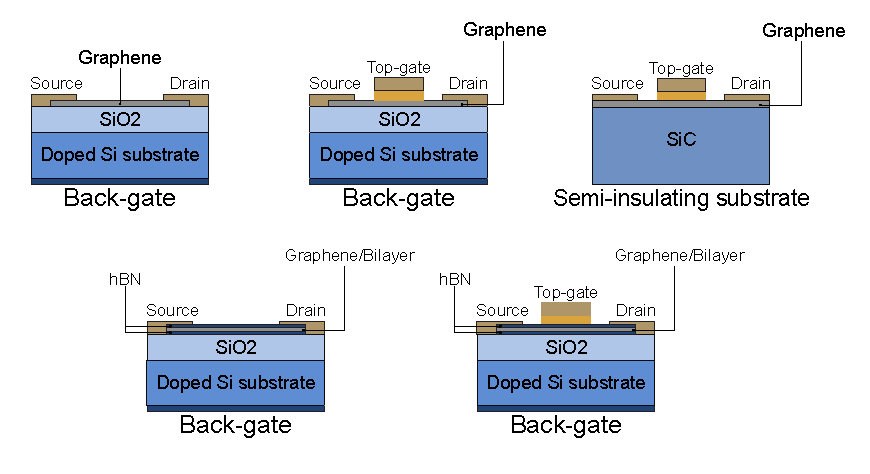
\includegraphics[width=\textwidth]{chapter_introduction/figures/graphene_device.pdf}
        \caption[Graphene Device Architectures and Operating Schematic]{
            \textbf{top,} Architectures of graphene \glspl{MOSFET}. Charge carriers can be modulated in a graphene channel (epitaxial, CVD-grown, or multi-layer) connecting two metal contacts by either a back-gate or a top-gate. SiC substrates have been used for growing in-situ thermally decomposed graphene, which has found successful radiofrequency applications.
            \textbf{bottom,} Same architectures can be now fabricated with graphene between two \gls{hBN} layers. Adapted from~\cite{schwierz2010graphene}.
        }
        \label{fig:intro:graphene_device}
    \end{center}
\end{figure}
%
These results were explained by: (1) an assumption that graphene has electrons with negligible effective mass close to the Fermi energy, and (2) a lack of direct carrier backscattering because of graphene's lattice symmetry~\cite{wolf2014graphene}. Although some believed scatterings due to charged impurities~\cite{hwang2007carrier} or microscopic ripples~\cite{schedin2007detection} to be predominant at low temperatures, weak electron--phonon scattering even at room temperature is considered to be responsible for the extrordinary mobility $\mu^{\text{in}}\simeq\SI{200000}{\centi\metre\squared\per\volt\per\second}$ reported from graphene sandwiched between two \gls{hBN} layers~\cite{morozov2008giant} (Fig.~\ref{fig:intro:graphene_device}). Having a slight lattice mismatch (about 1.5\%~\cite{giovannetti2007substrate}) relative to graphene, $\varepsilon_{\text{hBN}}\simeq$\numrange{3}{4}, and significant bandgap (\SI{5.9}{\electronvolt}), \gls{hBN} is considered the best insulating to encapsulate graphene, and indeed hBN-sandwiched graphene devices have been recently used for groundbreaking results such as unconventional superconductivity in bilayer graphene~\cite{cao2018unconventional} and Stoner ferromagnetism~\cite{seiler2021quantum}.

The high mobility alone is, however, insufficient. As we have mentioned earlier, one of the main motivations for engineering graphene-based transistors is that, because of the absence of electron backscattering, they should be robust against increases in off-state current when the \gls{CMOS} channel is scaled down~\cite{schwierz2013graphene,young2009quantum,katsnelson2006chiral}. Furthermore, the device conductance must be regulated by the gate voltage $V_textrm{G}$, and has to be robust against any voltage fluctuations. The figure of merit associated with last requirement is the so-called $I_\text{on}/I_\text{off}$. The on--off ratio quantifies the ability of any circuit component in electrical contact with the transistor to distinguish between the transistor's on and off-states. A high on--off ratio corresponds, typically, to a low leakage current.

\begin{figure}[hbtp]
    \begin{center}
        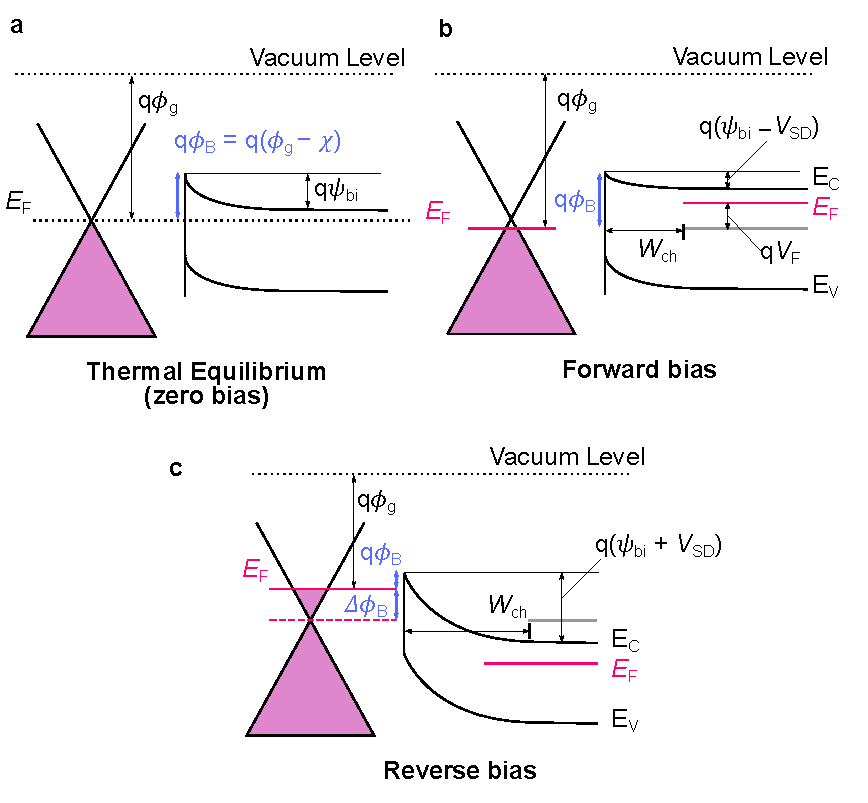
\includegraphics[width=\textwidth]{chapter_introduction/figures/operation_graphene.pdf}
        \caption[Graphene MOSFET Band Structure]
        {
            \textbf{a--c,} Energy-band diagrams of graphene--semiconductor contacts (a) in thermal equilibrium, (b) when a forward bias is applied, and (c) when a reverse bias is applied. $\chi$ is the electron affinity, $\psi_\textrm{bi}$ is the built-in potential, and $W_\textrm{ch}$ is the channel length~\cite{DiBartolomeo2016}.
        }
        \label{fig:intro:operation_graphene}
    \end{center}
\end{figure}

It is possible to estimate the on--off ratio of a device using the thermoionic-emission model for the drain current (see pictorial representation in Fig.~\ref{fig:intro:graphene_device}). When graphene is in contact with a semiconductor, the two work functions $\phi_\textrm{Si}$ and $\phi_\textrm{g}$ align accordingly based on the doping and the carrier concentrations. If $\phi_\textrm{Si} = \phi_\textrm{g}$, the \gls{SB} formed at the Si--graphene junction may be written as $\phi_B=E_g/2$, where $E_g$ is the semiconductor bandgap, and the on--off ration is~\cite{kim2011role}:
%
\begin{equation}\label{eq:bandgap_current_ratio}
    \frac{I_\textrm{on}}{I_\textrm{off}}\propto\exp{\frac{E_g}{2k_\textrm{B}T}},
\end{equation}
%
where $k_\textrm{B}T$ is the thermal energy. Some researchers suggest that bandgap values of \SIrange{0.3}{0.5}{\electronvolt} are ideal for \gls{CMOS} applications~\cite{schwierz2010graphene, reddy2011graphene}.

Despite considerable efforts, researchers have been hindered by the metallic nature of graphene from producing \gls{CMOS} architectures with high-resistance off-states, and have therefore deemed it unsuitable for logic applications. In contrast, graphene-based electronics are broadly useful in applications requiring high frequencies. For analogue applications, properties such as ballistic transport, linear current--voltage characteristics, high transconductance, and exceptionally high sustained currents ($> 10^8$ \si{\ampere\per\square\centi\metre}) have proven to be ideal~\cite{meric2008rf, meric2008current}.

\subsection{High-Frequency Applications}

The frequency device performance are characterised in terms of two quantities, namely cutoff $f_\textrm{T}$ and maximum of oscillations $f_\textrm{max}$ frequencies. The former indicates how quickly a signal may travel from the gate to the drain of the device and is often measured when the small-signal current gain approaches unity, while the latter is the highest possible frequency at which there is a non-vanishing power gain~\cite{schwierz2010graphene}.
The frequency response is inversely related to the length of the gate and proportional to the transconductance, which is approximately proportional to mobility\footnote[2]{This is strictly valid if the mobilities are in the diffusive regime. If carriers approach ballistic values, then the transconductance is constant.}. Therefore, to achieve high cut-off frequencies in a transistor, researchers must maintain high carrier mobility when the channel length is scaled down~\cite{schwierz2013graphene}. In this regard, numerous research groups have demonstrated \gls{RF} applications for graphene~\cite{colmiais2022towards, liao2012graphene, lin2009operation}.

Late in 2008, it was claimed that the first device with a cutoff frequency in the gigahertz region was fabricated using exfoliated graphene placed on a high-resistivity silicon substrate, with a \SI{30}{\nano\metre}-thick top-gate dielectric made of \ce{HfO2} and a \SI{500}{\nano\metre}-long gate~\cite{meric2008rf}. Despite a reported cutoff frequency of about $f_\textrm{T}\simeq\SI{14.7}{\giga\hertz}$ it was stated that excessive contact resistances and gate lengths were the primary causes of low ($f_\textrm{max}<\SI{1}{\giga\hertz}$) maximum frequency performance. The following year, Pd/Au contacts and a \SI{12}{\nano\metre}-thick aluminum oxide were implemented in a \SI{350}{\nano\metre}-long graphene gate, and although the cutoff frequency was increased to \SI{50}{\giga\hertz} the maximum frequency was increased only to \SI{2}{\giga\hertz}~\cite{lin2009development}. This poor performance was attributed to the organic contaminations on the graphene surface resulting from the use of poly(methyl methacrylate) (PMMA) as a supporting layer during the transfer process, as well as poor development of gate dielectrics~\cite{jang2014improved}.

After two years, a one-order-of-magnitude rise in the cutoff and the highest frequency of oscillation was demonstrated~\cite{lin2010100}. The devices are realised with an epitaxially grown silicon-carbide--graphene \glspl{MOSFET} with a \SI{240}{\nano\metre} gate length, Ti/Pd/Au contacts, and \ce{HfO2} \SI{10}{\nano\metre}-thick as top gate. Local gating is frequently preferred as gate-source, and gate-drain capacitances are inversely proportional to the channel length and minimised in this geometric configuration, hence improving the cut-off frequency that can be reached~\cite{liao2012graphene}. In addition to $f_\textrm{T}\simeq\SI{100}{\giga\hertz}$, the highest maximum frequency ever measured was $f_\textrm{max}\simeq\SI{100}{\giga\hertz}$, beyond the capabilities of any technology at the time. \citeauthor{xu2016contacts} noticed that, since the maximum oscillation frequency significantly depends on  device layout and parasitic resistances arising from the metallic contacts, partial passivation of the metal contacts and a multi-finger gate layout would be viable strategies to increase $f_\textrm{max}$~\cite{xu2016contacts}.

Later the same year, a \SI{144}{\nano\metre}-long gate device with $f_\textrm{T}\simeq\SI{300}{\giga\hertz}$ was developed using mechanically exfoliated graphene and \ce{Co2Si}–\ce{Al2O3} nanowire as self-aligned multi top-gates~\cite{liao2010high}. This result was also confirmed by comparison to the predicted value based on the relationship\footnote[2]{$f_\textrm{T} = g_\textrm{m}/(2\pi C_\textrm{g})$~\cite{sze2021physics}} between dc transconductance, gate capacitance, and the cutoff frequency in the case where total input parasitic capacitance is negligible. The authors did not report the power $G^{1/2}_\textrm{max}$, only the current gain $\abs{h_{21}}$, making it difficult for others to assess the $f_\textrm{max}$ of the device. A rough estimate might be extracted by looking at the results reported by Cheng and colleagues on a similar device, where the gate was built using a stack of Au/Ti/\ce{Al2O3}~\cite{cheng2012high}.

Improvements in the cutoff frequency response ($f_\textrm{T}\simeq\SI{427}{\giga\hertz}$ for a channel length of 67 nm) compared with that of \gls{CVD} graphene devices with similar gate length, however, were eclipsed by only minor improvements to the device maximum frequency response ($f_\textrm{max}=\SI{8}{\giga\hertz}$) when the gate length was lowered to \SI{46}{\nano\metre}. As for the cutoff frequency, it is vital to minimise all parasitic resistances and capacitances in order to optimise $f_\textrm{max}$. In addition, the output conductance must be decreased in order to obtain the highest feasible operating speeds, which is often accomplished by operating the transistor when the drain current is saturated.

Furthermore, researchers of IBM investigated on the saturation behavior of short-channel graphene transistors leveraging CVD graphene transferred to diamond-like and SiC substrates, in an attempt to improve the power gain~\cite{wu2012state}. These are particularly attractive possibilities since the substrates are commercially accessible on high-quality wafers, which makes it quite straightforward to scale up graphene arrays. Since the work function of graphene ($\phi^\textrm{g} = \SI{4.5}{\electronvolt}$) is greater than that of silicon carbide ($\phi^{\ce{SiC}} = \SI{3.7}{\electronvolt}$), negative charges accumulate on the graphene side of the contact, leaving graphene n-doped~\cite{sonde2009electrical}. The authors compensated this unwanted doping by using an innovative technique involving plasma-enhanced CVD silicon nitride as an intrinsic, p-type gate dielectric.

The transistors perform well at high speeds, not only because of their good cutoff frequencies ($f_\textrm{T}\simeq \SI{350}{\giga\hertz}$), but also because of their twofold increase in maximum oscillation frequency  $f_\textrm{max}$ $\simeq\SI{40}{\giga\hertz}$, suggesting undoped graphene substrates as ideal for high frequency applications. To the best of my knowledge, the current graphene transistor power-gain record is approximately \SI{70}{\giga\hertz}, achieved by using a ($0\,0\,0\,\overline{1}$) carbon-terminated surface of silicon carbide instead of the conventional (0\,0\,0\,1) Si. This indicates that a low contact resistance between the gold contacts and graphene is the primary factor responsible for the high maximum frequency~\cite{guo2013record}.

In terms of cutoff frequencies, the performance of graphene-based devices is comparable to that of the leading solid-state competitors, such as GaAs high-electron-mobility transistors (HEMT), InP HEMT, and Si \glspl{MOSFET}. The performance in terms of maximum frequencies, however, is one or two orders of magnitude below the required values for a competing technology~\cite{tan1990InGaAs, post2006RF,lai2007sub}. In the scientific literature, one of the most commonly cited underlying factors for this behaviour is the weak saturation in the drain current in graphene, which ultimately depends on the lack of a bandgap in the channel. Because of their intrinsic semiconductivity, graphene-derived materials such as nanoribbons and carbon nanotube-\glspl{MOSFET} could be a viable solution to this problem. In the following sections, I will investigate some important aspects of the electronic response at the device level for each class of materials.

\section{Carbon Nanotube Electronics}\label{intro:sec:cnt}

\co{Introduction: define your aims and objectives}
The literature on carbon nanotubes is vast and well documented. In the following, I have two primarily aims. Firstly, I will provide a comprehensive review of \glspl{CNTFET}, highlighting crucial elements that have, in my opinion, played a significant role in enhancing the competitiveness of nanotube-based transistors. Secondly, I will quantify the performance in order to compare it to \gls{GNR}-based transistors.

In contrast to graphene, \glspl{CNT} have an electrical bandgap that varies according to the nanotube chirality and diameter~\cite{dresselhaus2000carbon}, and may be defined in real space by two unit vectors $\vect{a_1}$ and $\vect{a_2}$ and any linear combination of these with integer coefficients, which are typically labelled $m$ and $n$~\cite{dresselhaus1998physical}. Depending on these coefficients, a \gls{CNT} can be metallic, quasi-metallic, or semiconducting. As depicted in Fig.~\ref{fig:intro:cnt_structure}, states resulting from quantisation in the circumferential direction may or may not pass through one of the $\vect{K}$ points in the first Brillouin zone of graphene, and the resulting \gls{CNT} will be metallic when the electronic states cross a $\vect{K}$ point, else it will be semiconducting. Exceptions to this simple rule arise from to the strong curvature when the diameter of the tube is sufficiently small, which leads to large spin--orbit interactions~\cite{steele2013large,laird2015quantum}.

\begin{figure}[hbtp]
    \begin{center}
        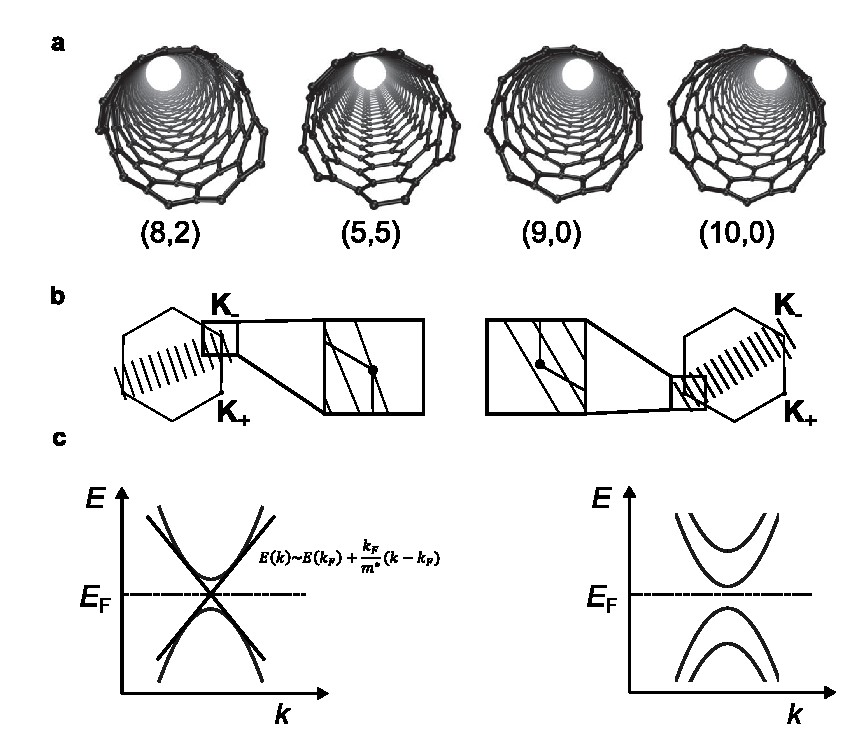
\includegraphics[width=\textwidth]{chapter_introduction/figures/cnt_structure.pdf}
        \caption[Carbon Nanotube Structure and Energy Dispersion]
        {
            \textbf{a}, Cartoon structure of a chiral (8, 2), an armchair (5, 5), and a zigzag (10, 0) nanotube.
            \textbf{b}, Graphene Brillouin zone and allowed \vect{k}-vectors for the (8, 2) and (10, 0) CNTs. A metallic tube (left) includes one of the \vect{K} points among the set of allowed \vect{k}-vectors. As shown in \textbf{c}, it is then possible to linearise the energy dispersion in the momentum space for low excitations (close to the Fermi energy $E_\textrm{F}$). Conversely, the \vect{K} point is not an allowed vector for semiconducting nanotube, and this leads to an energy gap. Inspired by~\cite{torres2014introduction}.
        }
        \label{fig:intro:cnt_structure}
    \end{center}
\end{figure}

The discovery of charge-carrier modulations within a nanotube produced by a gate-induced electric field was the first landmark which started the field~\cite{tans1998room}. These early \glspl{FET} were fabricated using a doped silicon substrate as the gate to tune the energy bands, with thermally grown silicon dioxide acting as the dielectric between the nanotube and the substrate, and Au contacts to electrically contacting the nanotube.

Since then, several \gls{CNTFET} designs have been put forward (Tab.~\ref{intro:tab:cnt_devices}), which may be even classified more fundamentally as devices with or without a spacer. The length of the spacer $L_\textrm{spr}$ is the gap between the channel and the metal contacts. Given that a certain class of nanotubes is intrinsically semiconducting, the flow of charge carriers in spacer-less devices is not generated by the electric field $\CMcal{E}_\textrm{SD}$ in the conductive channel, but rather by the concentration gradient of charges that exists between the two ends of the nanotube.

\begin{table}[]

    \centering
    \small

    \caption{\label{intro:tab:cnt_devices} Figures of merit for a few \glspl{CNTFET} reported in the literature. $SS$: subthreshold swing; $g_\textrm{m}$: intrinsic transconductances; $L_\textrm{ch}$: channel length; $\mu$: carrier mobility; $f_T$: cutoff frequency; $f_\textrm{max}$: maximum of oscillations frequency}

    \begin{tabular}{ccccccccc}
        \toprule
        \textit{Device}            & $I_\textrm{on}/I_\textrm{off}$ & $SS$       & $g_\textrm{mt}$                       & $L_\textrm{ch}$         & $f_T$~[$f_\textrm{max}$]~ & Ref.                        \\
        \textit{type}              &                                & (mV/dec)   & (\si{\micro\siemens\per\centi\metre}) & (nm)                    & (GHz)                     &                             \\
        \midrule
        \multirow{9}*{Bottom gate} & 10$^4$                         & 94         & $\simeq40$                            & 9                       & ---                       & ~\cite{Franklin2012}        \\
                                   & 10$^5$                         & $\simeq85$ & 40                                    & 15                      & ---                       & ~\cite{Franklin2010}        \\
                                   & 10$^5$                         & $\simeq85$ & 20                                    & 20                      & ---                       & ~\cite{Franklin2010}        \\
                                   & $10^5$                         & 60         & 20                                    & 200                     & ---                       & ~\cite{weitz2007high}       \\
                                   & 10$^5$                         & $\simeq63$ & ---                                   & 200                     & ---                       & ~\cite{Lin2005}             \\
                                   & 10$^4$                         & 80         & 50                                    & 240                     & ---                       & ~\cite{Javey2004}           \\
                                   & ---                            & ---        & 143                                   & 800                     & ---                       & ~\cite{chimot2007gigahertz} \\
                                   & 10$^4$                         & ---        & ---                                   & $1500$                  & 1.5 -- 3.0                & ~\cite{schroter2016cntfet}  \\
                                   & ---                            & 70         & 12$^\dag$                             & $\num{2000}^\ddagger$   & ---                       & ~\cite{javey2002high}       \\
                                   & $10^8$                         & ---        & ---                                   & $<\num{10000}^\ddagger$ & ---                       & ~\cite{Derenskyi2014}       \\
                                   & ---                            & ---        & $-500$                                & ---                     & 30                        & ~\cite{le2007intrinsic}     \\

        \midrule
        \multirow{3}*{Top gate}    & $10^6$                         & ---        & 20$^\dag$                             & 80                      & ---                       & ~\cite{javey2005high}       \\
                                   & 2                              & ---        & $\simeq50$                            & 100                     & 25                        & ~\cite{che2013t}            \\
                                   & 50                             & ---        & 310                                   & 100                     & $\simeq70$ [80]           & ~\cite{cao2016radio}        \\
                                   & ---                            & ---        & 0.3                                   & 210                     & ---                       & ~\cite{Nihey2002}           \\
                                   & $10^5$                         & ---        & 33.5                                  & \num{85000}             & ---                       & ~\cite{Lau2013}             \\

        \bottomrule
    \end{tabular}

    \begin{tabbing}
        $^\dag$Normalized by the tube width.\\
        $^\ddagger$Referred to the gated length of a nanotube. \\
    \end{tabbing}

\end{table}

The role of the gate is to lower the energy barrier between the metal and the semiconducting channel, thereby allowing electrons to tunnel from the source through the \gls{SB}. In this case, both the metal $\phi^\textrm{M}$ and the \gls{CNT} $\phi^\textrm{CNT}$ work functions are critical in the transistor performance: the lower their mismatch is, the more efficient is the injection of the carriers at the source, resulting in current densities that approach the Ohmic-contact case (Tab.~\ref{intro:tab:cnt_performance}). In contrast, \glspl{CNTFET} with spacers are not limited by the at-the-source injection step, since the electric field $\CMcal{E}_\textrm{SD}$ drives the carriers flow, and indeed \citeauthor{javey2009carbon} produced a device with spacers where the mismatch between $\phi^\textrm{M}$ and \gls{CNT} $\phi^\textrm{CNT}$ was large, and found that the device was more resistant to ambipolar conduction because of the substantial energy barrier at the drain~\cite{javey2009carbon, torres2014introduction}.

\begin{table}[]
    \caption{\label{intro:tab:cnt_performance}Comparative analysis of the most common electrical-contact types for connecting \glspl{CNTFET}~\cite{singh2015comparative}. Applied drain voltage $V_\textrm{SD} = \SI{0.5}{\volt}$}
    \centering
    \small
    \begin{tabular}{ccccccccc}
        \toprule
        \textit{Contact}  & $I_\text{on}$ & $I_\text{off}$ & $I_\text{on}/I_\text{off}$ & $g_\text{mt}$         & $SS$     & \\
        \textit{type}     & (A)           & (A)            &                            & (\si{\micro\siemens}) & (mV/dec) & \\
        \midrule
        Conventional      & \num{1.4e-5}  & \num{4.1e-10}  & \num{3.4e4}                & 29                    & 100        \\\Tsmall
        Partial S/D-doped & \num{1.5e-5}  & \num{2.3e-8}   & \num{6.4e2}                & 64                    & 93         \\\Tsmall
        Schottky-Barrier  & \num{3.3e-6}  & \num{2.3e-8}   & \num{1.4e2}                & 20                    & 110        \\\Tsmall
        Tunnel            & \num{5.5e-6}  & \num{1.2e-8}   & \num{4.8e2}                & 13                    & 108        \\
        \bottomrule
    \end{tabular}
\end{table}

There is another reason to study how different work functions affect the transistor performance. Solid-state semiconductors have dangling bonds at the surface resulting in Fermi-level pinning, which means that the variation of the band bending is independent of the metal work function even when large~\cite{sankey1984si}. Since, ideally, the \gls{CNT} structure has no open bonds, the Fermi level of the metal will not be pinned to mid-gap states~\cite{bachtold2001logic, svensson2009dependence}. For example, it has been shown that metals with high work functions, such as Pd ($\phi^\textrm{Pd}\simeq$ \SIrange{5.2}{5.6}{\electronvolt}), yields p-type behavior with high on state current for large-enough \gls{CNT} diameter $d_\textrm{CNT}\ge\SI{2}{\nano\metre}$~\cite{leonard2000role}, and that the \gls{SB} height is inversely proportional to $d_\textrm{CNT}$~\cite{svensson2009dependence}. The reason for this observation was explained within the \gls{SB} framework, i.e.\ large work functions prevent the minority carriers to hop over the barrier back into the channel, resulting in low leakage current. Metals with large work functions are, however, more strongly associated with large contact resistances when their wettability is poor~\cite{lim2009contact}, suggesting mentals with good wettability such as Ti and Cr as ideal for low contact resistances.

Often, however, metals with low work functions and good wettability have a strong tendency to oxidise, especially in air. A possible workaround is to cap low work function contacts all-around with metals having high work functions, such as Sc and Y~\cite{ding2009contacted}: the \glspl{CNTFET} produced with such contacts reported high on-state currents ($I_\textrm{on}\simeq\SI{250}{\micro\ampere}$), mobilities $\mu\ge\SI{500}{\cm\square\per\V\per\second}$, and \gls{DIBL} up to \SI{105}{\si{\mV\per\V}}, together with excellent switching behaviour $SS\simeq\SI{73}{\milli\volt}$~dec$^{-1}$~\cite{ding2009contacted,peng2019carbon}.

The subthreshold swing $SS$ measures the rate at which the gate voltage switches on the transistor, and it is a metric that quantifies the control the gate has on the conductive channel. Furthermore, it is often indirectly linked to heat dissipation, which, as we have mentioned in Sec.~\ref{intro:sec:motivation}, is one the primary obstacles to miniaturising \gls{CMOS} technology. Since the carriers are thermally injected, it is challenging to reduce the operating voltage while at the same time improving CPU operational speed and maintaining a low off-state power dissipation. Since the off-state power is scales quadratically with the off-state current $P_\textrm{off} = RI^2_\textrm{off}$, the objective is to lower the $I_\textrm{off}$ without sacrificing $I_\textrm{on}$. The process of thermally injecting charge carriers imposes a limit, called Boltzmann limit, on the subthreshold slope which for the is approximately $2.3 k_\textrm{B}T/q\simeq\SI{60}{\milli\volt}$~dec$^{-1}$ at room temperature.

One of the most promising approaches to overcoming the Boltzmann limit uses a different source--carrier injection mechanism based on Zener tunneling rather than thermal means. If the transmission probability does not depend on the energy gap between the metal and the nanotube work functions, but instead depends on the interband tunneling, the output current is temperature-independent. Several researchers have proposed both \gls{CNT}- and \gls{GNR}-based transistors with this operating mechanism~\cite{ionescu2011tunnel, hammam2018sub, hwang2019room}.

Crucial is also the conduction type. The vast majority of the \gls{CNTFET} transfer $I_\textrm{SD}$--$V_\textrm{G}$ characteristics reported are p-doped~\cite{allen2007carbon}, and this is largely because (1) photochemical resists in the lithographic steps often leave p-type contaminations on the substrate~\cite{nosho2005n}, and (2) oxygen impurities~\cite{nonoguchi2016simple}. Instead, n-type devices would be desirable.

As a result of the presence of electron-donating dopants, n-type doping assures that, in a heterojunction, \glspl{CNT} do not have to pull electrons from the opposite side of the junction because this need is satisfied by the dopant atom~\cite{brownlie2018advances}. Instead, the nanotube would preferentially donate electrons to the heterojunction p-type side, leaving behind an electron vacancy (hole) that is stabilised by the excess of negative charge carriers provided by the dopant.

An interesting solution for fabricating n-type \glspl{CNTFET} is by doping the nanotube-channel surface with elements of the first two groups of the periodic table, such as \ce{K+} and Mg$^{2+}$~\cite{bockrath2000chemical, zhou2000modulated}. Precise control of the doping density per \gls{CNT} unit length is, however, necessary, and this is often difficult because of the high tendency of \glspl{CNT} to aggregate when dispersed in solution, often yielding uncontrolled doping levels~\cite{brownlie2018advances, yu2012air}. Additionally, ionised impurities, instability in air and to temperature fluctuations have hampered the applications of n-type \glspl{CNTFET}.

\subsection{Channel Length Scaling}

Whether Si could operate at channel lengths below \SI{10}{\nano\metre} was a question for a long time, but recent scientific advances in FinFETs~\cite{yang20045nm} and Gate-All-Around FETs~\cite{gu2011first} have demonstrated its viability and fostered a plethora of commercial uses (currently, modern devices employ the \SI{4}{\nano\metre} technology). Nonetheless, \gls{CMOS} scaling has always been a good-enough reason for investigating fabrication techniques and materials robust against short-channel effects\footnote[2]{Typicaly short-channel effects are threshold voltage roll-off, off-state leakage current, and channel length-modulation are just a few of the problems}.

\begin{figure}[hbtp]
    \begin{center}
        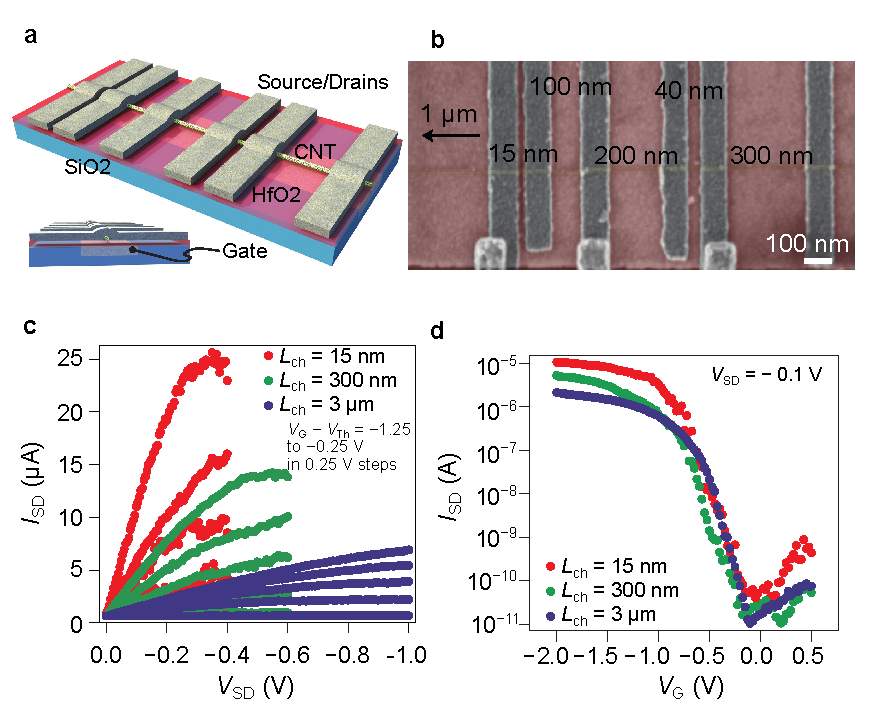
\includegraphics[width=\textwidth]{chapter_introduction/figures/scaling_channel_length.pdf}
        \caption[High-$\kappa$ Carbon Nanotube Field-Effect Transistors]{
            \textbf{a}, Schematic of the set of transistors used by \citeauthor{franklin2010length}. Cleverly, a single \gls{CNT} was used with $L_\textrm{ch}$ ranging from $\SI{1}{\micro\metre}$ downo to $\SI{15}{\nano\metre}$.
            \textbf{b}, False-coloured SEM image.
            \textbf{c}, Output $I_\textrm{SD}$--$V_\textrm{SD}$ characteristics, demonstrating improvement in the on-state current when $L_\textrm{ch}$ is scaled from $\SI{3}{\micro\metre}$ down to $\SI{15}{\nano\metre}$.
            \textbf{d}, Subthreshold $I_\textrm{SD}$--$V_\textrm{G}$ transfer curves, showing the consistency of $V_\textrm{Th}$ and $SS$ when $L_\textrm{ch}$ is reduced by more than two orders of magnitude. Adapted from~\cite{franklin2010length}.
        }
        \label{fig:intro:cnt_device_1}
    \end{center}
\end{figure}

In \glspl{CNTFET}, two are the main device parameters that can be scaled down: the contact length $L_\textrm{c}$ and the channel length $L_\textrm{ch}$. The $L_\textrm{ch}$ scaling typically reduces the gate control over the channel, hence the ability of the electric field generated through the gate to bend the silicon band structure. Intuitively, as the channel length is reduced, the electric field created by the source contact will be felt by the charge carriers more and more. \Glspl{CNT} may provide a suitable platform for such scaling because of their ultrathin, hollow nature. This could be, however, a double-edged sword. Since the electron effective mass is smaller\footnote[4]{$m^*_\textrm{CNT} = (0.228 \pm 0.129)m_0$~\cite{marulanda2008carrier}} compared to that of silicon, the tunneling probability may be large enough to increase drastically the source--drain current. From a device performance point of view, this often means an increase in the $SS$ and high $I_\textrm{off}$.

\Citeauthor{franklin2010length} conducted one of the earliest systematic studies on $L_\textrm{ch}$ scaling, through a series of experiments on \glspl{CNT}~\cite{franklin2010length} (Fig.~\ref{fig:intro:cnt_device_1}). When the channel length was reduced by more than two orders of magnitude (from \SI{3}{\si{\micro\metre}} down to \SI{15}{\si{\nano\metre}}), a consistent trend was found in both the threshold voltage ($V_\textrm{Th}\simeq\SI[separate-uncertainty = true]{-0.5(0.2)}{V}$) and subthreshold swing ($SS\simeq\SI{90}{\milli\volt}$~dec$^{-1}$). The threshold voltage is the gate voltage required to fully invert the semiconductor. It is typically measured by applying a small $V_\textrm{SD}$ and measuring the $I_\textrm{SD}$ as a function of $V_\textrm{G}$, provided that the drain current is at least one order of magnitude smaller than the applied gate voltage, scaled accordingly by the gate capacitance.

This, essentially, means that the gate-generated electric field controls the carriers flow even when the electric field between source and drain become non-neglibile. An aggressive reduction of the channel length, however, could in principle make the gate less effective in controlling the charge carriers, meaning that larger gate variations are required for pulling the same amount of current from the drain.
This essentially implies that the gate-generated electric field controls the flow of carriers even when the electric gradient between source and drain is no longer negligible. However, an extreme reduction of the channel length might, in theory, reduce the current amplification (the gain), excluding the possibility of employing \glspl{CNT} as molecular op-amp.

And indeed, at that time of \Citeauthor{franklin2010length}'s, experiment part of the scientific community believed that the $L_\textrm{ch}$ scaling could have a negative impact on the \glspl{CNTFET} gain, i.e. low transconductance $g_\textrm{m}$~\cite{avouris2003carbon,javey2009carbon, anantram2006physics}. In a standard \gls{MOSFET}, the transconductance $g_\textrm{m}$ is defined as $g = \partial{I_\textrm{SD}}/\partial{V_\textrm{G}}$, and it is measured by applying a small, constant bias. Typical values lies in the range \qtyrange[range-units = bracket]{1}{30}{\milli\siemens\per\micro\metre} for a small-signal field-effect transistor~\cite{sze2021physics}. However, Franklin and his colleagues measured transconductance values as high as \SI{40}{\micro\siemens\per\micro\metre} for \glspl{CNTFET} with $L_\textrm{ch}\simeq\SI{15}{\nano\metre}$ ((Fig.~\ref{fig:intro:cnt_device_2})), which corresponds to transconductance values of approximately \qtyrange[range-units = bracket]{91}{110}{\milli\siemens\per\micro\metre}, thereby meeting the requirements for a technology compatible and competitive with the silicon.

\begin{figure}[hbtp]
    \begin{center}
        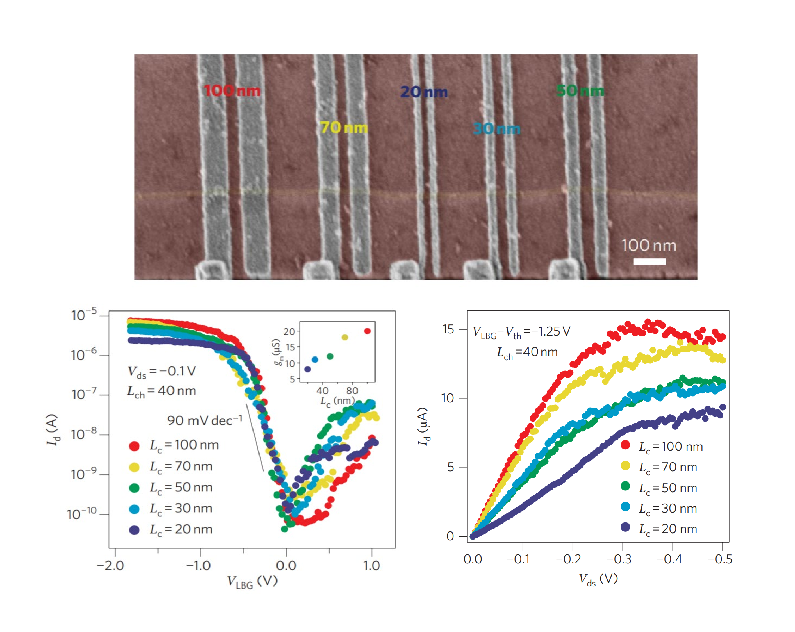
\includegraphics[width=\textwidth]{chapter_introduction/figures/cnt_device_2.pdf}
        \caption[Contact Length Scaling in Carbon Nanotube Field-Effect Transistors]
        {
            Top frame is the false-coloured SEM image of several transistors on the same nanotube but having different $L_\textrm{c}$, from \SIrange{100}{20}{\nano\metre}. Even for the smaller contacts the gate has complete control over the channel and the device switches quicker than most Si \glspl{MOSFET}-based competitors. Small contact leghts, however, severly degrades the on-state current, although the saturation regime it is still well within the experimental accessible region. Adapted from~\cite{franklin2010length}
        }
        \label{fig:intro:cnt_device_2}
    \end{center}
\end{figure}

Two years after their findings, \Citeauthor{Franklin2012} shrank the channel length of a \gls{CNTFET} to less than 10 nanometers~\cite{Franklin2012}. Their technique involved the use of smaller tubes, and a reduction of the \gls{EOT} to \SI{0.65}{\nano\metre}: this was achieved by wrapping the nanotube in a all-around gate (Fig.~\ref{fig:intro:cnt_device_3}). The rationale behind the use of all-around gates is that if the oxide is extremely thick, the gate control over the flow of carriers in the channel tends to weaken~\cite{sze2021physics}. The length of the channel was successfully lowered from down to \SI{9}{\nano\metre}, and the authors reported on-current values close the ballistic limit for transistors \SI{41}{\nano\metre}~\cite{franklin2010length}. \citeauthor{franklin2010length} advocated for decreasing the \gls{CNT} diameter to reduce the subthreshold swing and off-current with minimum effect to the on-current, and

\begin{figure}[hbtp]
    \begin{center}
        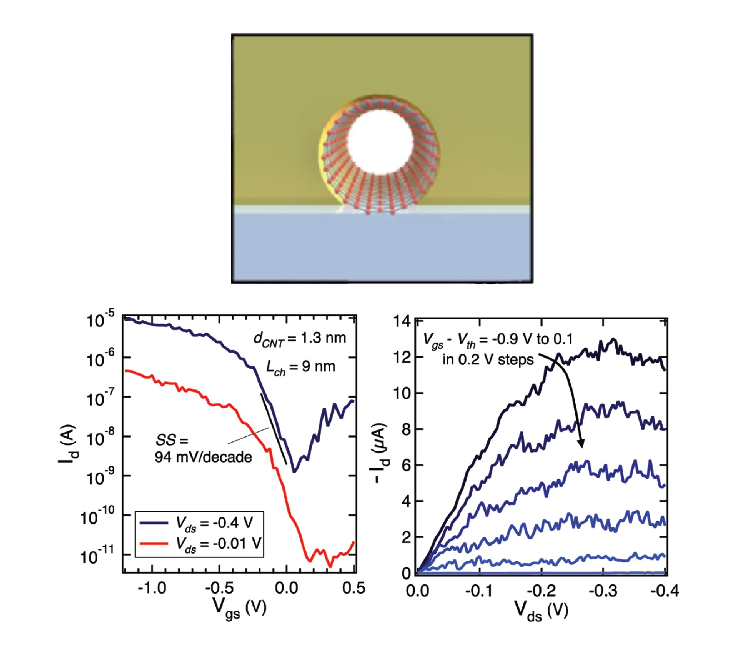
\includegraphics[width=\textwidth]{chapter_introduction/figures/cnt_device_3.pdf}
        \caption[Channel Length Scaling in Carbon Nanotube Field-Effect Transistors]
        {
            \textbf{top}, Visualisation of all-around gate and hollow \gls{CNT} structures
            \textbf{bottom left}, Subthreshold (off-state) and, \textbf{bottom right} output (on-state) characteristics for a $L_\textrm{ch}\simeq\SI{9}{\nano\metre}$ demonstrates that the gate does not loose control over the channel. Adapted from~\cite{Franklin2012}.
        }
        \label{fig:intro:cnt_device_3}
    \end{center}
\end{figure}

in fact also the switching performance ($SS\simeq\SI{94}{\milli\volt}$~dec$^{-1}$) generated great enthusiasm around the \gls{CNT} technology, leading the year after to the first proposal of carbon nanotube computer~\cite{shulaker2013carbon}.

As previously pointed out, in order to keep the off-current low, not only the channel width must be sufficiently wide to discourage quantum tunneling across the barrier, but also has to be large enough to prevent thermal hopping above the barrier, limiting the back-injection of minority carriers into the channel. We have already seen one device parameter that may be used to adjust this value, namely the nature of the electrical connections. In the following part, we will briefly examine another other adjustable parameter, namely the contact length $L_\textrm{c}$.

\subsection{Contact Length Scaling}
When \glspl{MOSFET} are shrank down to the nanoscale, one must consider also the effect played by the overlap of the \gls{CNT} with source and drain. Numerical investigations of this phenomenon have suggested that high contact transparencies might result when the metal--\gls{CNT} coupling is weak, meaning the electronic states of the tube are, more or less, unchanged after the formation of the lead--\gls{CNT} junctions~\cite{fediai2015electron, teichert2019improved, fediai2016towards}. Especially for long contacts ($L_\textrm{c}\simeq\SI{30}{\nano\metre}$), one suggestion advanced by these studies was that in order to achieve high contact transparencies one should minimize coupling while maximising the overlap region, and that the junction Pd--\gls{CNT} might leads to quasi-Ohmic contacts~\cite{liu2017scaling}.

By using the transfer length\footnote[2]{The transfer length is the distance over which a fraction equal to $1-e^{-1}$ of the total current is \textit{transferred} from the contact metal to the semiconducting channel ($e$ is the Euler's number), and it is frequently used as a metric for quantifying the coupling between electrical contacts and conduction channel (small transfer lengths result in greater couplings, and, consequently, lower contact resistances)~\cite{saraswat2021materials}.} model, experiments performed on small-diameter ($d_\textrm{CNT}\simeq\SI{1.5}{\nano\metre}$) \glspl{CNT} highlighted inverse scaling of the contact length with the resistance between the nanotube and the electrodes, i.e.\ $L_\textrm{c}\propto1/R_\textrm{c}$~\cite{purewal2007scaling, franklin2010length}. These observations were rationalised by considering dipole moments building up at the metal--\gls{CNT} interface~\cite{leonard2000role}, which are likely caused by interface states at the junction

A large density of dipole charges should then translates into a large density of interface states, which could pin the Fermi level. Since in a planar contact, the dipole in a metal--\gls{CNT} contact is localised in all directions, the consequence of having interface states is that the \gls{CNT} energy bands might be shifted away from the junction, inducing the formation of a narrow barrier responsible for the increased contact resistance~\cite{svensson2011schottky}. Therefore, in order to limit the band shift from the junction, electrical contact with work functions close in value to the \gls{CNT} one might protect reduce the Fermi-level pinning caused by surface states.

More sophisticated computational methods have also been used attempting at clarify the nature (and the role) of the chemical bonds produced when the \gls{CNT} interacts with the electrode crystal structure. By applying \gls{NEGF} numerical schemes, \citeauthor{fediai2016towards} suggested that the most unfavourable length scaling should be observed for weakly-interacting metals such as Cr, Pd, Pt, and, on the other hand, metals such as Au, Al, and Sc could be nearly insensitive to the scaling of $L_\textrm{c}$ when it is decreased down to $\approx\SIrange{15}{20}{\nano\metre}$~\cite{fediai2016towards}. Furthermore, the authors proposed a numerical criterion through which they projected a better contact resistance scaling for Rh in comparison to Au, Pt, and Pd. However they also simulated the metal--junction long limit and suggested that differences in the $R_\textrm{c}$ resulted by adopting Pd instead of Rh were neglibile, suggesting that the better scaling for the Rh--\gls{CNT} junctions may be not worth the cost of the material.

% Schematic energy levels in the same quantum dot potential for two limits of dispersion and confinement
% discussed in the text. Electron correlations are not consired. Superimposed on the level diagram are wave function envelopes for several electron shells. Mode index is indicated for the first three shells. (b) Sequence of Coulomb blockade peaks measured in a quantum dot of length


\section{Single-Electron Conduction}

At cryogenic temperatures, the smearing of $k_\textrm{B}T$ makes a number of quantum phenomena observables. Examples of such are the conductance blockage due to strong Coulomb interactions~\cite{Averin1986}, interference effects~\cite{stojetz2005effect}, periodic shell-filling signatures related to the tunneling through energy levels~\cite{sapmaz2005electronic}, and Kondo effects originated from the hybridisation of \gls{CNT} spin states with the continuum of states in the metallic leads~\cite{jarillo2005orbital}. Because the energy scales for such quantum effects typically increase with decreasing the system size $L$ (see also Ch.~\ref{ch:theory}), a great deal of these effects have been experimentally observed in \glspl{CNT}.

\begin{figure}[hbtp]
    \begin{center}
        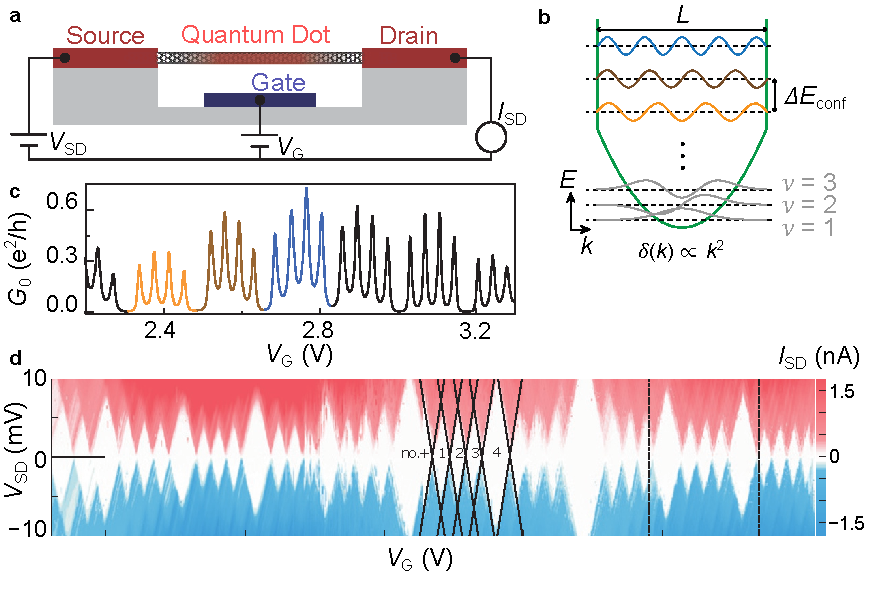
\includegraphics[width=\textwidth]{chapter_introduction/figures/cnt_set.pdf}
        \caption[Carbon Nanotube Single-Electron Transistors]
        {
            \textbf{a}, \Gls{QD} device schematic. A \gls{CNT} is contacted by source and drain electrodes and capacitively coupled to a gate. The current $I_\textrm{SD}$ through the device is measured as a function of $V_\textrm{SD}$ and $V_\textrm{G}$. Through $V_\textrm{G}$, one may control the number of electrons $N$ on the island and tune the dot energy levels.
            \textbf{b}, \Gls{QD} energy levels schematic (electron--electron interactions are ignored). Electronic wave function envelopes $\psi(k)$ are superimposed on the level
            diagram for several electron shells. With $\nu$ we indicate the mode index for the first three shells. Adapted from~\cite{laird2015quantum}.
            \textbf{c}, Coulomb blockade peaks sequence measured in \gls{QD} whose length
            is $L\simeq\SI{750}{nm}$. Peaks corresponding to three successive shells are colored to illustrate the connection to different wave functions. Although the four electrons
            that fill each shell occupy states of similar energy, an extra energy
            $\delta$ is needed to populate a higher shell, leading to fourfold periodic peak spacing. Adapted from~\cite{sapmaz2005electronic}.
            \textbf{d}, Experimental device that confirmed the fourfold periodicity. White diamonds are regions where the $I_\textrm{SD}$ is suppressed because of Coulomb blockade. Adapted from~\cite{leturcq2009franck}.
        }
        \label{fig:intro:cnt_set}
    \end{center}
\end{figure}

The platform most commonly used in quantum transport experiments is an electronic device made by \gls{CNT} embedding a \gls{QD} (Fig.~\ref{fig:intro:cnt_set}a). The exact position of the \gls{QD} inside \gls{CNT} has been object of scientific debate, but it is now considered to be the nanotube portion between the large \gls{SB} barriers arising at the metal--\gls{CNT} junctions, where electrons can be trapped by the electric fields induced by local gates located beneath the tube~\cite{laird2015quantum}. A \gls{QD} (or, more generally, a \gls{SET}) can be realised if the contact resistances at the junctions source--\gls{QD} and \gls{QD}--drain exceed a certain limit, i.e.\ $R_\textrm{c}\ge\SI{26}{\kilo\ohm}$~\cite{likharev1999single}; when the contacts are such opaque they are tipically called \textit{tunneling barriers}, given that the only transport mechanism through which current can flow thorugh the \gls{QD} is quantum tunneling. \Gls{CNT} energy levels can then be studied by measuring the $I_\textrm{SD}$ through such \glspl{QD} as a function of $V_\textrm{SD}$, $V_\textrm{G}$, and other parameters such as magnetic field $B$, temperature $T$, etc.


\subsection{Carbon Nanotube Quantum Dots}

We will take a deeper look in Ch.~\ref{ch:theory} about theoretical technicalities, here we will limit ourselfs to briefly overview the energy scales involved in quantum transport experiments. The energy required to add a single electron to the \gls{QD}, $e^2 / 2 C$, where $C$ is the dot capacitance, must be greater than the thermal energy $k_{\mathrm{B}}T$. Given that total capacitance values are $C\sim\SI{1e-18}{\farad}$ and energy scales $E_{\mathrm{C}}, \Delta$ up to the meV range, single-electron charging effects are manifested as Coulombd bloackade (Fig.~\ref{fig:intro:cnt_set}d) which allow full mapping of discrete charge states and, for high-quality devices, excited states and exotic multibody interactions~\cite{hanson2007spins, laird2015quantum}.


\co{Franck--Condon}

Since the introduction of tunneling barriers add a longitudinal confinement, the impact that the \gls{CNT} mechanical motion have on the electronic transport has been studied both theoretically and experimentally. Particularly interesting were the experimental evidences collected by \cite{leturcq2009franck} on suspended \gls{CNT} by using a slightly modified architecture compared to the one reported in Fig.~\ref{fig:intro:cnt_set}a. The \gls{QD} was precisely embedded between the source and the drain by using a second, top gate combined with a standard \ce{Si}/\ce{SiO2} backgate.

\begin{figure}[hbtp]
    \begin{center}
        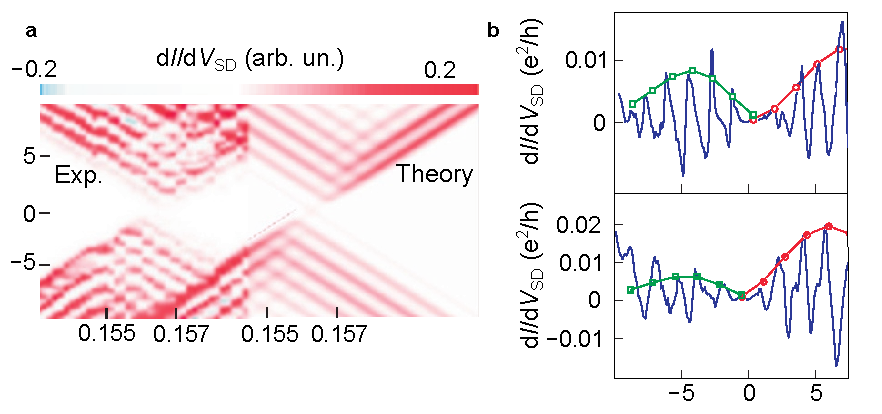
\includegraphics[width=\textwidth]{chapter_introduction/figures/cnt_FC.pdf}
        \caption[Carbon Nanotube Single-Electron Transistors]
        {
            \textbf{a}, Experimental and theoretical zoom into a part of \gls{CNT} Coulomb diamonds, showing the suppression of the low-bias conductance. In order to reproduce the experimental evidence, \citeauthor{leturcq2009franck} used a value for the electron--vibron coupling $\gamma=3.3$.
            \textbf{b}, Differential conductance measured at $V_\textrm{TG}=\SI{0.068}{\volt}$ (top) and $V_\textrm{TG}=\SI{0.157}{\volt}$ (bottom). Solid lines are fits of the conductance maxima using the Franck--Condon progression. \textbf{top}, $g=3.5$ (negative bias voltage, green squares) and $g=5.0$ (positive bias voltage, red circles). Deviations from the progression were explained by the researchers as due to electronic excited states within the $V_\textrm{SD}$ window. \textbf{bottom},  $g=3.0$ (green squares) and $g=4.5$ (red circles). Adapted from~\cite{leturcq2009franck}.
        }
        \label{fig:intro:cnt_FC}
    \end{center}
\end{figure}

The exceptional quality of the samples allowed the researchers the unambiguous observation of several features, such as (1) excited vibronic states as lines running paralles to the edges of the Coulomb diamonds, (2) the appearance of absorption sideband peaks within the Coulomb blockaded regions when $T$ was increased, and (3) an aggressive suppression of the current at the edge of the diamonds. Since the current at the edges was suppressed by an amount comparable with the current magnitude for the excited vibronic states, the researchers hypothesised the Franck--Condon conductance blockade~\cite{koch2005franck, koch2006theory}.

\subsection{Luttinger-Liquid}

In interacting 1D systems such as \gls{CNT}, the electrons behaviour cannot be captured within the Fermi liquid theory, but by Luttinger-liquid models~\cite{egger1997effective, egger1999luttinger,kane1997coulomb}. In these models, spin and charge excitations are described as bosonic modes, are separable, and propagate at different velocities. Furthermore, the electron--electron interaction leads to a \gls{TDOS} suppression and interaction-dependent power laws for transport quantities.
The experimental evidence of such interactions was revealed through a series of remarkable experiments first on individual \gls{CNT} bundle (also called \textit{rope}), i.e.\ multiples tubes closely packed together and later on single \gls{CNT}.

\begin{figure}[hbtp]
    \begin{center}
        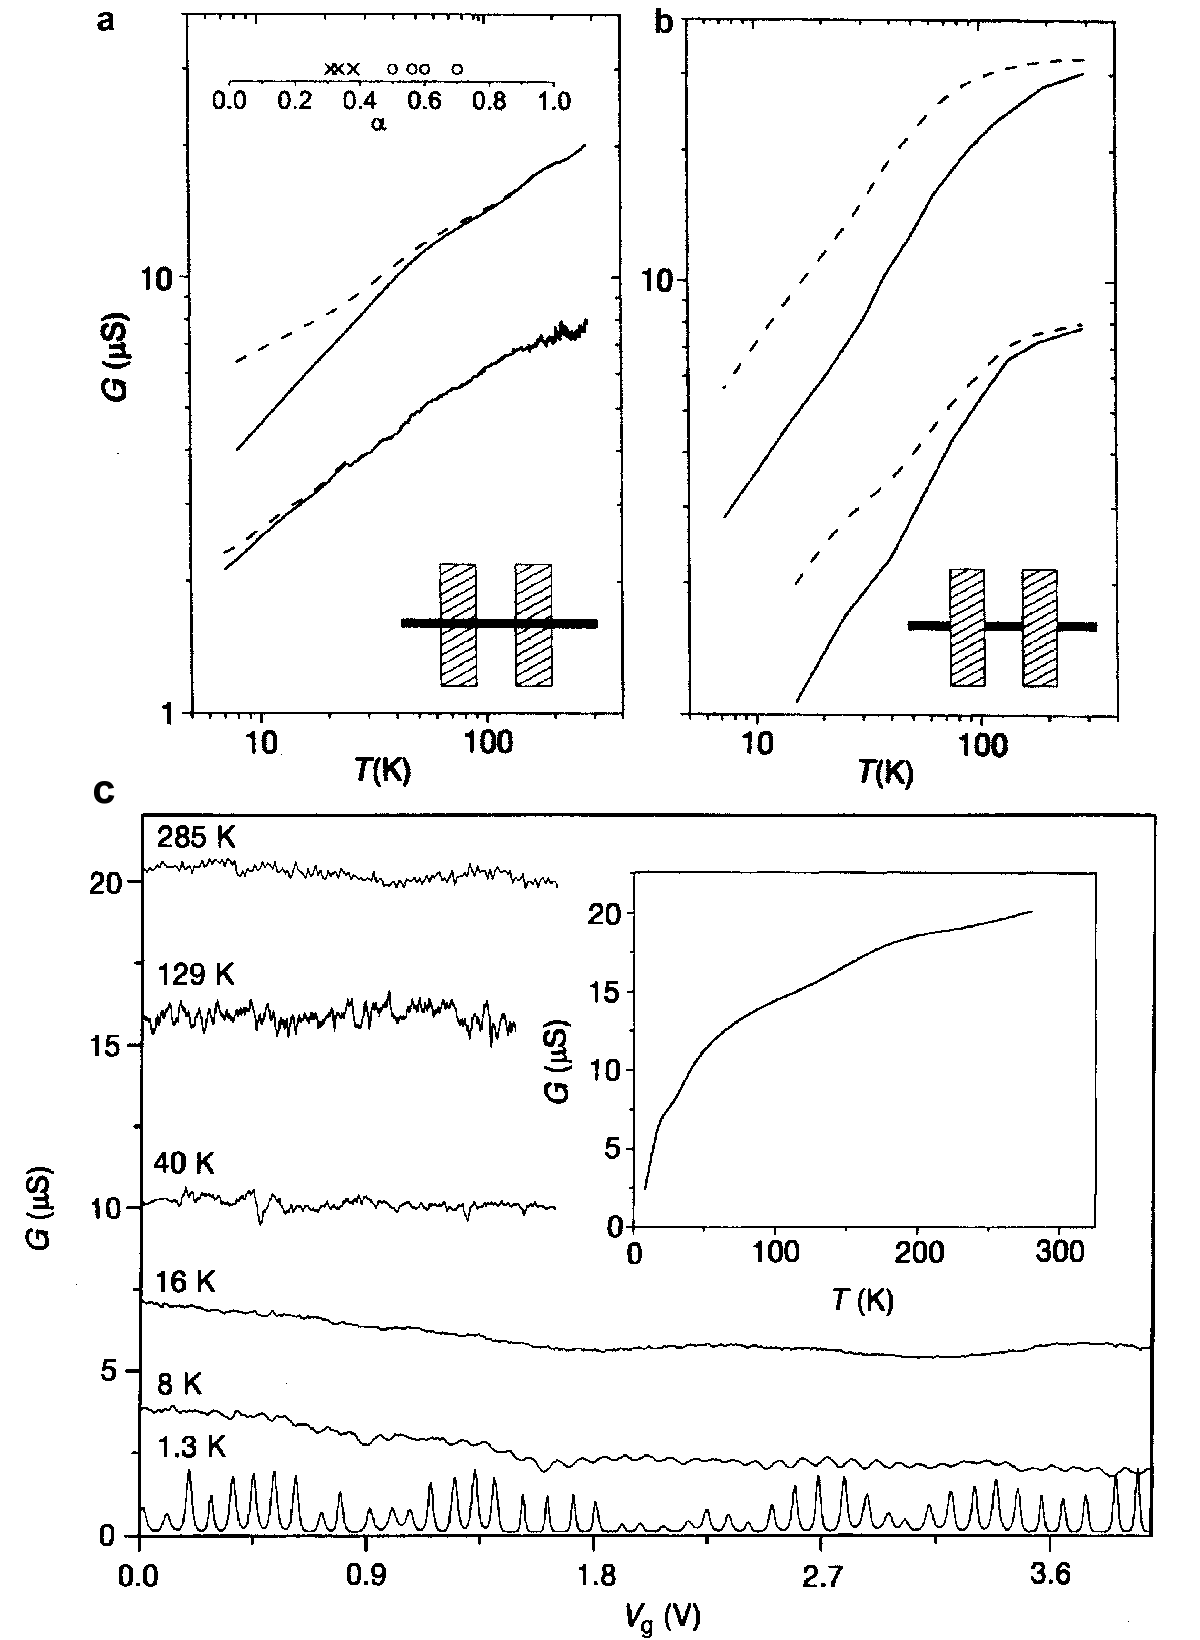
\includegraphics[width=\textwidth]{chapter_introduction/figures/bocrath_LL.png}
        \caption[Luttinger-Liquid in Ropes of Carbon Nanotubes]
        {
            \textbf{a}, Bulk-contacted and \textbf{b}, end-contacted nanotube ropes, showing raw data (solid line) and data scaled by the temperature dependence expected from the Coulomb blockade model (dashed line).
            \textbf{c}, Two-terminal temperature-dependent conductance for metallic bulk-contacted ropes. Adapted from~\cite{bockrath1999luttinger}.
        }
        \label{fig:intro:bocrath_LL}
    \end{center}
\end{figure}

One of such experiments, for instance, was performed by \citeauthor{bockrath1999luttinger} on carbon nanotubes ropes contacted either from the top (end-contact) or from below (contacting the tube along its bulk)~\cite{bockrath1999luttinger}. In both cases, researchers found a power-law scaling of the conductance measured at zero bias as the temperature was increased, i.e.\ $G(T) \sim T^\alpha$. The phenomenological interpretation of the exponent $\alpha$ the author gave was that, depending on the fabrication details, the power law exponent may change. In particular, they reported an $\alpha_{\text{end}}\simeq 0.6$, whereas in the case of bulk contact the suppression of the \gls{TDOS} is weaker, setting an $\alpha_{\text{bulk}}\simeq 0.3$. Comparing these values with the expected electron--electron interaction predicted by the theory yielded a $g\simeq 0.28$.

The Luttinger parameter, $g$, which characterizes the strength and sign of the electron interaction, can be related to readily measured nanotube parameters $E_{\mathrm{C}}$, the charging energy, and $\Delta$ the mean orbital level spacing by $g=\left(1+2 E_{\mathrm{C}} / \Delta\right)^{-1 / 2}$.

\begin{figure}[hbtp]
    \begin{center}
        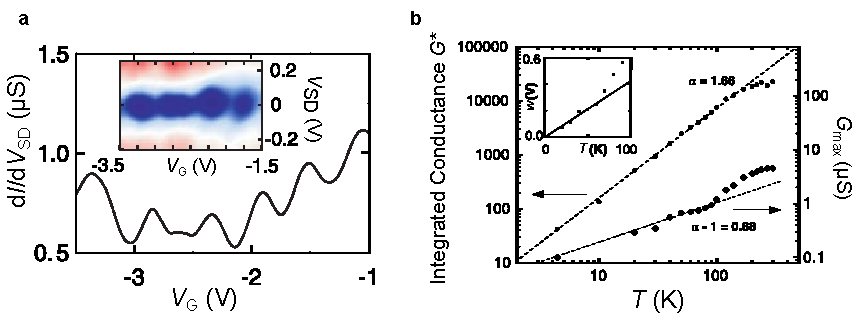
\includegraphics[width=\textwidth]{chapter_introduction/figures/cnt_postma.pdf}
        \caption[Luttinger-Liquid in Ropes of Carbon Nanotubes]
        {
            \textbf{a}, Oscillations in $G$ at \SI{260}{\kelvin}, showing Coulomb bloackade. (Inset) Differential conductance map. Blue regions represents low conductance, red regions high conductance. The authors did not report the colorbar.
            \textbf{b}, Temperature-dependent conductance $G$ (right axis) and integrated conductance $G^*$ (left axis) reveal a power law scaling for the tunneling through the nanotube, explained within the Luttinger-liquid framework. (Inset) At low temperature, the peak width $w$ correlates linearly with $T$. Adapted from~\cite{postma2001carbon}.
        }
        \label{fig:intro:cnt_postma}
    \end{center}
\end{figure}

Further experimental evidences, however, demonstrated that the interpretation of the tunneling exponent may be not that trivial.  Postma et al. measured the conductance of electrons tunneling inside a carbon nanotubes QD where the tunneling barriers were introduced by mechanically bending the nanotube with an AFM tip. Since the \gls{QD} was not end-contacted they explained the conductance-suppression exponent as the result of a tunneling event from a Tomonaga--Luttinger liquid (the nanotube) into a Luttinger island (the quantum dot hosted inside the tube). In this case, the conductance was strongly suppressed, reporting an $\alpha_{\text {bulk }} \sim 0.64$, and rationalised by strong electron--electron interactions $g\sim0.23$ as expected from theory~\cite{egger1999luttinger}. This observation was hypothesised to be the consequence of a different kind of tunneling mechanism called \textit{correlated sequential tunneling}~\cite{thorwart2002correlated}. Briefly, in this mechanism the once the electron tunnel on the \gls{QD} it does not immediately tunnels onto the drain but there is a dephasing due to interaction with plasmon modes.









% An exciting area opened by this work is the possibility to combine the spin degree of freedom with mechanical and optical degrees in clean, suspended nanotubes.
% There has already been progress in engineering quantized phonons in nanotubes and studying their interactions with the charge on quantum dots (Benyamini et al.,
% 2014; Huttel et al., 2009; Lassagne et al., 2009; Sapmaz
% et al., 2005a; Sazonova et al., 2004; Steele et al., 2009a).
% Evidence for the discreteness of longitudinal stretching
% phonon modes, comes from Frank-Condon blockade in
% suspended nanotubes (Leturcq et al., 2009x`'; Sapmaz et al.,
% 2005a), discussed theoretically by (Flensberg, 2006; Mariani and von Oppen, 2009; Sapmaz et al., 2003). By
% tuning the discrete phonon modes away from resonance
% with qubit splittings, long qubit lifetimes may be achievable. On the other hand, when the qubit splitting is
% nearly resonant with a discrete phonon mode, coherent energy exchange should be possible between them,
% in a solid-state analog of cavity quantum electrodynamics (P´alyi et al., 2012). Strong spin-phonon coupling in
% suspended nanotubes may also enable enhanced sensing
% of nanotube motion (Ohm et al., 2012).






\section{Concluding Remarks and Thesis Outlook}

% Graphene nanoribbons exhibit intriguing physical and chemical properties not only for technological advancement in areas where graphene and carbon nanotubes lack performance, but also for the physics they can reveal. At this time, bottom-up graphene nanoribbons have demonstrated remarkable transport and exotic properties, but these have been studied solely on the synthesis substrate. Attempting to investigate these properties at the device level will be one of the next major obstacles in the nanoribbon field. At this time, these evidences are largely unavailable and unclear.

% There are three roles to which graphene nanoribbons may technologically contribute. The first application is that of sensors. Given the ability to functionalise the edges with a variety of chemical substituents, a large number of studies in various gas atmospheres have demonstrated excellent selectivities and good flexibility. A second possible field could be the integration in low-power devices, where by reducing required supply voltages, ribbons with lower bandgaps and consequently higher mobilities could be employed. A third and more enthusiastic application would be the development of decoherence-tolerant quantum hardware utilising their topological properties.

From the discussion developed in this chapter it is evident that while the electronic properties of carbon nanotubes have been explored in detail, and their possible usage in
quantum systems has been defined, there is still no clarity about the role of vibrational states and the consequences that large length/width ratio may have on \glspl{GNR}. In addition, whereas carbon nanotubes have demonstrated disappointingly short spin-coherence times, graphene nanoribbons exhibit edge-states coherence times of up to \si{\micro\second} at room temperature. As a result, interest in their potential applications in quantum devices has tremendously grown.

In the following, we provide an outline for the thesis structure. The purpose of this work is to tackle current challenges when using \glspl{MGNR} for transport experiments, and in particular  try to answer to the unanswered question on how to engineer competitive \gls{GNR}-based electronic devices.
We begin with a general theoretical introduction of \glspl{GNR}, based on their crystal structure and electronic properties. We then discuss mesoscopic scale systems and their properties, and we will give a more in depth overview of the main transport regime when a nanoscopic system is contacted in a \gls{SET} fashion.

We will then introduce the peculiar physics of 1D systems, why they are different from other dimensionality, and why they are relevant in the study of \gls{MGNR} electronic properties. We will then introduce the fabrication methods we have used to engineer and optimise \gls{GNR}-based devices, followed by a discussion of the experimental techniques we have used to acquire the experimental data. In this respect, we will explain both \gls{DC} and \gls{AC} setup. We will also include the fabrication and the testing part of micro-Hall sensors made with Au and graphene that could be used in the future to measure anisotropy of \gls{GNR} functionalised with \gls{SMM}.

Three main projects are then presented in detail. We begin with the investigation of the temperature-dependent of the tunneling conductance through a single \gls{GNR}. This is the first of its kind study ever reported, and we shall critically discuss how these results can be collocated in the current literature, followed by why these results are relevant for several possible technological advancements. We then progress to study a particular strategy we have found to produce ultra-clean \gls{GNRSET}, allowing the first investigation of the effects of the coupling between quantized vibrational modes (vibrons) and electronic degrees of freedom in molecular \gls{GNR} quantum dots. Finally, we conclude by investigating two possible strategies for controlling the injection of dopants into \gls{MGNR}, i.e.\ by chemical functionalisation along the edges and by insertion of porphyrin rings carrying transition-metal ions inside the \gls{GNR} backbone.



% In interacting 1D systems such as CNT, the electrons behaviour cannot be captured within the Fermi liquid theory, but by Luttinger-liquid models. In this models, spin and charge excitations are described as bosonic modes, are separable, and propagate at different velocities. Furthermore, the electron--electron interactions lead to suppression of the \gls{TDOS} and interaction-dependent power laws for transport quantities.
% The presence of these interactions was tackled through a series of remarkable experiments first on carbon nanotubes ropes, i.e.\ multiples tubes closely packed together and later on single-walled carbon nanotubes.

% One of such experiments, for instance, was performed by Bockrath et al. [83] on carbon nanotubes ropes contacted either from the top (end-contact) or from below (contacting the tube along its bulk). In both cases, researchers found a power-law scaling of the conductance measured at zero bias as the temperature was increased, i.e.\ $G(T) \propto T^\alpha$. The phenomenological interpretation of the exponent $\alpha$ the author gave was that, depending on the fabrication details, the power law exponent may change. In particular, they reported an $\alpha_{\text {end }} \sim 0.6$, whereas in the case of bulk contact the suppression of the \gls{TDOS} is stronger, setting an $\alpha_{\text {bulk }} \sim 0.3$. Comparing these values with the expected electron--electron interaction predicted by the theory yielded a $g\sim0.28$.

% The Luttinger parameter, $g$, which characterizes the strength and sign of the electron interaction, can be related to readily measured nanotube parameters $E_{\mathrm{C}}$, the charging energy, and $\Delta$ the mean orbital level spacing by $g=\left(1+2 E_{\mathrm{C}} / \Delta\right)^{-1 / 2}$. 

% Further experimental evidences, however, demonstrated that the interpretation of the tunneling exponent may be not that trivial.  Postma et al. measured the conductance of electrons tunneling inside a carbon nanotubes QD where the tunneling barriers were introduced by mechanically bending the nanotube with an AFM tip. Since the \gls{QD} was not end-contacted they explained the conductance-suppression exponent as the result of a tunneling event from a Tomonaga--Luttinger liquid (the nanotube) into a Luttinger island (the quantum dot hosted inside the tube). In this case, however, although a higher electron--electron interaction was expected $g\sim0.23$ from the theory, the conductance was only mildly suppressed, reporting an $\alpha_{\text {bulk }} \sim 0.64$. This observation was hypothesised to be the consequence of a different kind of tunneling mechanism called \textit{correlated sequential tunneling}. Briefly, in this mechanism the once the electron tunnel on the \gls{QD} it does not immediately tunnels onto the drain but there is a dephasing due to interaction with plasmon modes.



% This device remarkably showed clear single-electron transistor behaviour up to 260 K, whereas a few later Cui et al. produce a working single-electron transistor at room temperature by local modification of thin CNT bundles.

% Room-temperature operating \gls{SET} are appealing devices not only because can be used in low-power applications but also are useful for the readout of pulsed-gate experiments and qubits. 

% In one dimension,The Fermi surface is not abrupt, even at zero temperature, and various power-law dependencies are expected in transport. This state is referred to as a Luttinger liquid $[81,82]$. Nanotubes are a nearly ideal realization of interacting electrons or holes in one dimension, and so provide an excellent testing ground for theoretical predictions of the behavior of Luttinger liquids, particularly in transport.

% Power-law scaling of the conductance $G=\mathrm{d} I / \mathrm{d} V_{\mathrm{Sd}}$ with temperature $T$ and source-drain bias $V_{\mathrm{Sd}}$, distinctive features of transport through a Luttinger liquid, has been observed in nanotubes in several experiments $[8,42, 83, 84].



